\section{Tarea}

\subsection{Problema propuesto: }

\begin{enumerate}[label={[\arabic*]}]
    \item Contar los números impares y menores de 20 de un vector de números enteros generados de forma aleatoria (la solución puede usar el método std :: count\_if ) 
    \item Diferencias, ventajas y desventajas de las clases QVector y QList. 
    \item Crear una interface gráfica (que implemente señales y slots) que muestre una lista de países, al dar clic sobre alguno que se muestre un Label o Text con el idioma y capital correspondiente.
\end{enumerate}




\section{Equipos, materiales y temas utilizados}

\begin{itemize}
    \item Subsistema de Windows para Linux (WSL) con Ubuntu.
    \item Sistema operativo: Microsoft Windows [Versión 10.0.26100.6584]
    \item TeX Live 2025
    %\item Strawberry Perl (requerido por MiKTeX para la ejecución de scripts auxiliares en la compilación de ciertos paquetes).
    \item Helix 25.01.1 (e7ac2fcd)
    \item Visual Studio Code 1.104.0 x64
    \item Git version 2.41.0.windows.1
    \item Cuenta activa en GitHub para la gestión de repositorios remotos.
    \item Qt Creator
    \item Leguaje de programación C++
    \item Librería Qt
\end{itemize}




\section{URL de Repositorio Github}

\begin{itemize}
    \item URL del Repositorio GitHub para clonar o recuperar.
    \item \url{https://github.com/yhuayhuahi/Teo.git}
    \item URL para el laboratorio (\itemPracticeNumber) en el Repositorio GitHub.
    \item \url{https://github.com/yhuayhuahi/Teo/tree/main/laboratorios/lab\itemPracticeNumber}
\end{itemize}




\section{Desarrollo de las actividades}

\subsection {\textcolor{red}{Actividad 01: Implementación en C++}}

\subsubsection {Función Main en C++}

A continuación se muestra la implementación de la función main en C++ que genera un vector de números enteros aleatorios y cuenta cuántos de ellos son impares y menores de 20 utilizando el método.

\begin{lstlisting}[style=cpp-style, caption={Función Main en cpp - Primera implementación}]
#include <iostream>
#include <vector>
#include <algorithm> // std::count_if
#include <cstdlib>   
#include <ctime>     

int main() {
    //para generar números aleatorios
    srand(static_cast<unsigned int>(time(nullptr)));

    // Generamos un vector de numeros enteros aleatorios
    std::vector<int> numeros;
    int n = 20;

    for (int i = 0; i < n; ++i) {
        numeros.push_back(rand() % 50); //números aleatorios entre 0 y 49
    }

    //mostramos los números generados
    std::cout << "Numeros generados a continuación: ";
    for (int num : numeros) {
        std::cout << num << " ";
    }
    std::cout << std::endl;

    // Contar cuántos son impares y menores de 20 ! usando count_if
    int conteo = std::count_if(numeros.begin(), numeros.end(), [](int x) {
        return (x % 2 != 0) && (x < 20);
    });

    std::cout << "Cantidad de numeros impares y menores de 20 encontrados: " << conteo << std::endl;

    return 0;
}
\end{lstlisting}



\subsubsection{Prueba de ejecución}

Se realizo la prueba de ejecución del código en C++ y se obtuvo el siguiente resultado:

\begin{figure}[H]
    \centering
    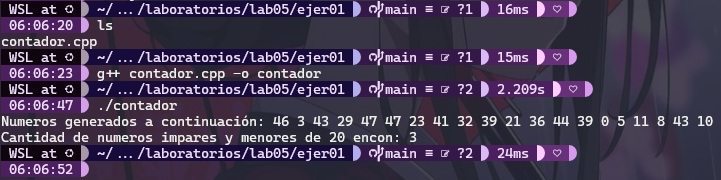
\includegraphics[width=0.9\textwidth]{img/Prueba01.png}
    \caption{Interfaz inicial de la aplicación Qt}
    \label{fig:qt_app}
\end{figure}




\subsection{\textcolor{red}{Actividad 02: Diferencias, ventajas y desventajas de las clases QVector y QList.}}

\subsubsection{Diferencias identificadas}

\textbf{Comportamiento por versión de Qt}

\begin{enumerate}
    \item Si se trabaja con Qt5, las diferencias todavía importan: QVector
    suele ofrecer mejor rendimiento para elementos grandes y acceso contiguo;
    QList puede comportarse distinto para tipos grandes (indirección). MIT Stuff
    \item Si se trabaja con Qt6, las diferencias son prácticamente nominales: la
    implementación es la misma/compatible y muchos de los viejos problemas de
    QList se resolvieron por unificación. Qt
\end{enumerate}

\textbf{Almacenamiento en memoria}

\begin{enumerate}
    \item Qt5: QVector<T> = elementos contiguos. QList<T> = en muchos casos elementos alocados individualmente y punteros en un array. 
    \item Qt6: ambos almacenan elementos de forma contigua, un comportamiento tipo std::vector.
\end{enumerate}

\textbf{Operaciones como prepend o append}

\begin{enumerate}
    \item Qt5: QList históricamente tenía mejor coste amortizado para prepend en ciertas implementaciones; QVector era más eficiente para crecimiento cuando se requiere memoria contigua. 
    \item Qt6: se añadió optimización de prepend a QList (y por tanto a QVector vía alias) para no romper expectativas. Qt
\end{enumerate}

\textbf{Compatibilidad y estilo de API}

\begin{enumerate}
    \item Muchas APIs de Qt históricamente devolvían QList; por eso se tuvo decisión de unificar para facilitar migraciones entre versiones y evitar confusión en la API pública.
\end{enumerate}



\subsubsection{Ventajas y desventajas (prácticas)}

\textbf{Ventajas de QVector:}

\begin{enumerate}
    \item Almacenamiento contiguo \(\to \) mejor localidad de caché \(\to \) mejor rendimiento para acceso secuencial/aleatorio. 
    \item Menos sobrecarga al almacenar tipos grandes (evita alocar cada elemento por separado).
\end{enumerate}

\textbf{Desventajas de QVector:}

\begin{enumerate}
    \item prepend() no era tan eficiente como en QList esto claro antes de las actualizaciones, dependiendo del uso concreto. 
    \item Estado (Qt6): alias de QList --- las diferencias previas desaparecen en gran medida.
\end{enumerate}

\textbf{Ventajas de QList:}

\begin{enumerate}
    \item API cómoda y era la recomendada por la documentación en muchos casos; en ciertas situaciones prepend() tenía mejor coste amortizado. Para tipos pequeños no siempre era peor; comportamiento dependía de sizeof(T) declaraciones como Q\_DECLARE\_TYPEINFO.
\end{enumerate}

\textbf{Desventajas de QList:}

\begin{enumerate}
    \item Para tipos no triviales o grandes, podía inducir muchas asignaciones individuales en el heap y pérdida de localidad de referencia → peor rendimiento y mayor uso de memoria. Por eso muchos desarrolladores preferían QVector como "default". 
    \item Estado (Qt6): implementación unificada, por lo que la mayoría de las desventajas históricas ya no aplican.
\end{enumerate}




\subsection{\textcolor{red}{Actividad 03: Implementación de una interfaz gráfica con Qt}}

\subsubsection {Implementación en C++ con Qt}

A continuación se muestra la implementación en C++ con Qt de una interfaz gráfica que muestra una lista de países y al dar clic sobre alguno se muestra un Label o Text con el idioma y capital correspondiente.

\begin{lstlisting}[style=cpp-style, caption={mainwindow.h}]
#ifndef MAINWINDOW_H
#define MAINWINDOW_H

#include <QMainWindow>
#include <QStringListModel>
#include <QMap>

QT_BEGIN_NAMESPACE
namespace Ui { class MainWindow; }
QT_END_NAMESPACE

class MainWindow : public QMainWindow
{
    Q_OBJECT

public:
    MainWindow(QWidget *parent = nullptr);
    ~MainWindow();

private slots:
    void on_countrySelected(const QModelIndex &index); // slot

private:
    Ui::MainWindow *ui;
    QStringListModel *model; // lista
    QMap<QString, QPair<QString, QString>> datosPaises; // pais -> (idioma, capital)
};

#endif // MAINWINDOW_H
\end{lstlisting}

\subsubsection {Implementación del archivo mainwindow.cpp}

\begin{lstlisting}[style=cpp-style, caption={mainwindow.cpp}]
#include "mainwindow.h"
#include "./ui_mainwindow.h"
#include <QStringList>

MainWindow::MainWindow(QWidget *parent)
    : QMainWindow(parent)
    , ui(new Ui::MainWindow)
{
    ui->setupUi(this);

    // lista de paises
    QStringList paises = {
        "Peru",
        "Mexico",
        "Colombia",
        "Argentina",
        "Chile",
        "Estados Unidos",
        "Canada",
        "Francia",
        "Italia",
        "Japon"
    };

    // idioma y capital
    datosPaises = {
        {"Peru", {"Español", "Lima"}},
        {"Mexico", {"Español", "Ciudad de Mexico"}},
        {"Colombia", {"Español", "Bogota"}},
        {"Argentina", {"Español", "Buenos Aires"}},
        {"Chile", {"Español", "Santiago"}},
        {"Estados Unidos", {"Ingles", "Washington D.C."}},
        {"Canada", {"Ingles y Frances", "Ottawa"}},
        {"Francia", {"Frances", "Paris"}},
        {"Italia", {"Italiano", "Roma"}},
        {"Japon", {"Japones", "Tokio"}}
    };

    // se crea el modelo y se asocia al QListView
    model = new QStringListModel(this);
    model->setStringList(paises);
    ui->listView->setModel(model);

    // conectamos la señal y slot
    connect(ui->listView->selectionModel(), &QItemSelectionModel::currentChanged,
            this, &MainWindow::on_countrySelected);
}

MainWindow::~MainWindow()
{
    delete ui;
}

void MainWindow::on_countrySelected(const QModelIndex &index)
{
    QString pais = model->data(index, Qt::DisplayRole).toString();

    if (datosPaises.contains(pais)) {
        QString idioma = datosPaises[pais].first;
        QString capital = datosPaises[pais].second;
        ui->labelInfo->setText("Idioma: " + idioma + "\nCapital: " + capital);
    } else {
        ui->labelInfo->setText("Informacion no disponible");
    }
}
\end{lstlisting}

\subsubsection{Pruebas de ejecución}

Se realizaron pruebas de ejecución para verificar que la interfaz gráfica funciona correctamente. Se seleccionaron diferentes países de la lista y se comprobó que la información mostrada en el Label o Text era la correcta.

\begin{figure}[H]
    \centering
    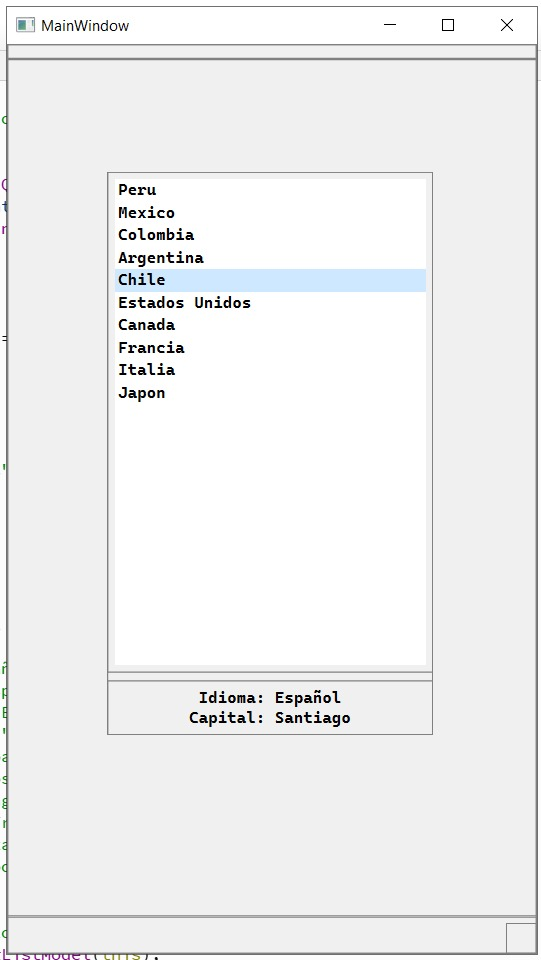
\includegraphics[width=0.6\textwidth]{img/Prueba02.jpg}
    \caption{Interfaz mostrando información de un país seleccionado}
\end{figure}

\begin{figure}[H]
    \centering
    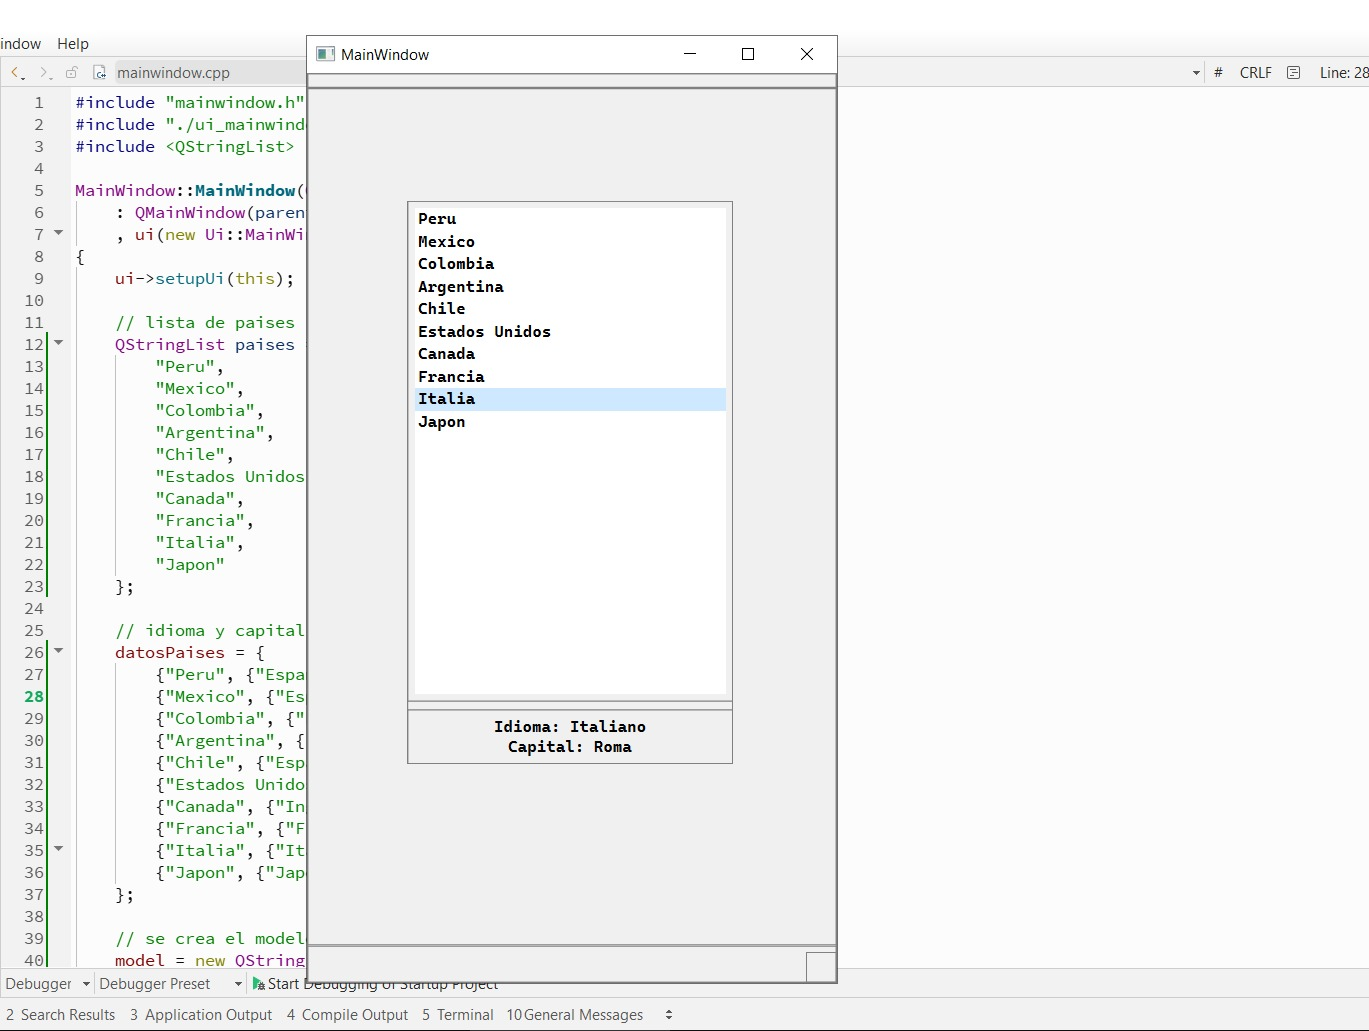
\includegraphics[width=0.8\textwidth]{img/Prueba03.jpg}
    \caption{Interfaz mostrando información de otro país seleccionado}
\end{figure}

\begin{figure}[H]
    \centering
    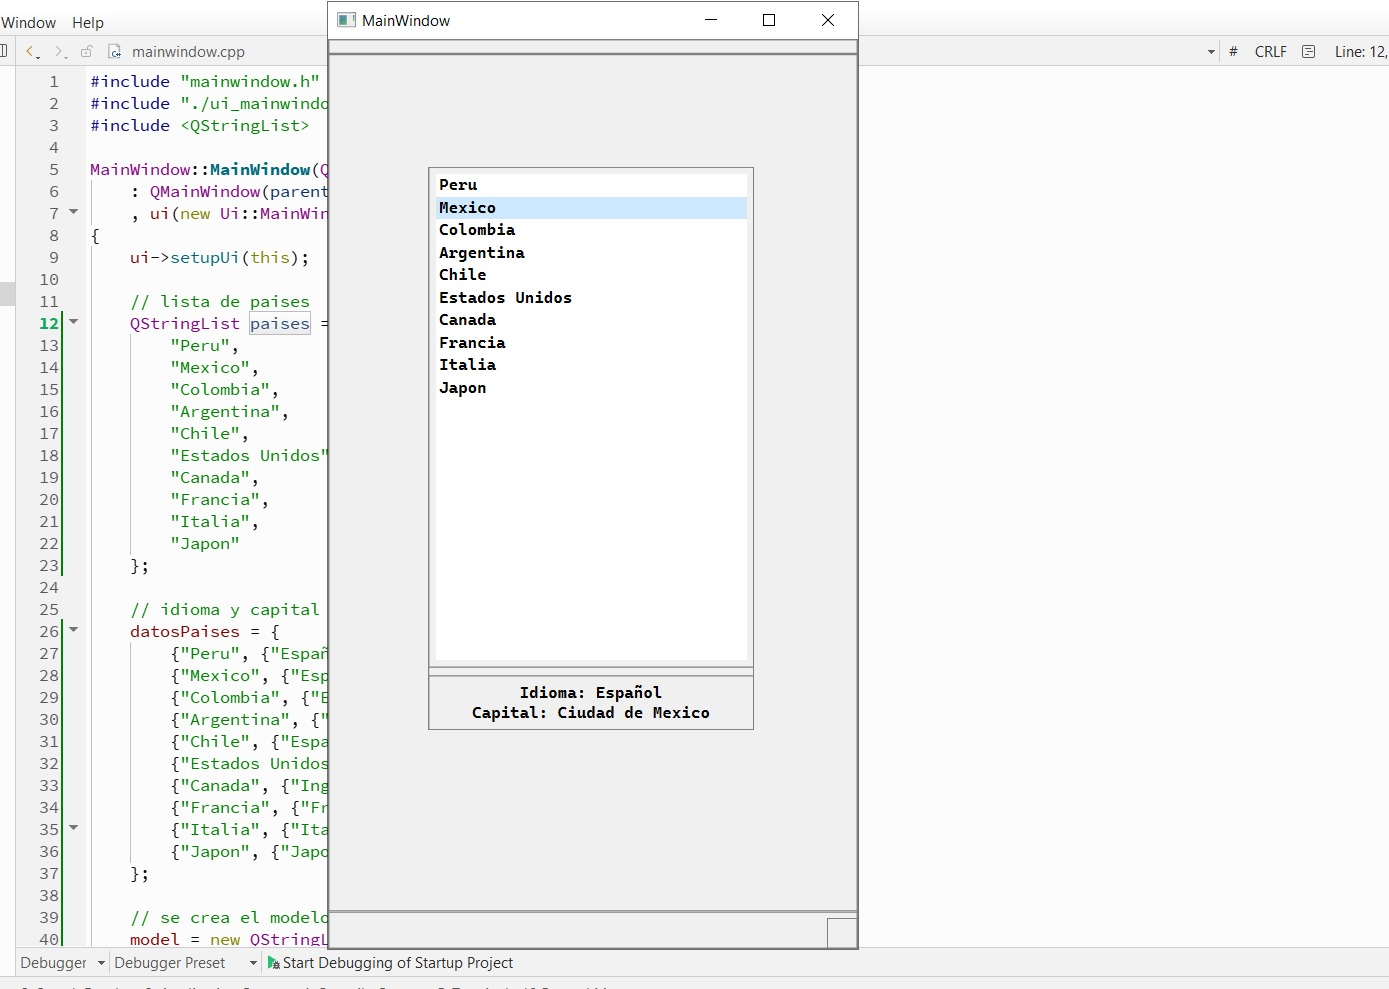
\includegraphics[width=0.8\textwidth]{img/Prueba04.jpg}
    \caption{Interfaz mostrando información de otro país seleccionado}
\end{figure}



\subsection {\textcolor{red}{Commits realizados}}

\subsubsection {Primer Commit}

\begin{itemize}
    \item Este commit se hizo despues de terminar la primera implementación de código para C++ con Qt para el ejercicio propuesto en el laboratorio. 
\end{itemize}

\begin{figure}[H]
    \centering
    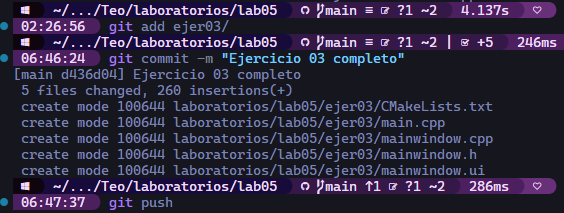
\includegraphics[width=0.8\textwidth]{img/Commit01.png}
    \caption{Primer Commit - Ejercicio 03 completo}
    \label{fig:commit1}
\end{figure}



\subsection {Estructura del laboratorio}

A continuación se muestra la estructura de archivos y carpetas del laboratorio realizado:
Claramente los archivos de compilación y otros que se pudieron generar no se subieron al repositorio.

\begin{figure}[H]
    \centering
    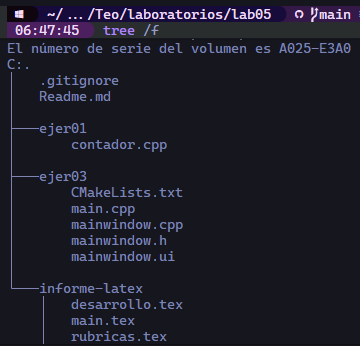
\includegraphics[width=0.8\textwidth]{img/Estructura.png}
    \caption{Estructura de archivos y carpetas del laboratorio}
    \label{fig:estructura}
\end{figure}



\section{Cuestionario}

\textbf{No hay un cuestionario para este laboratorio.}




